\documentclass{article}
\usepackage{gvv-book}
\usepackage{gvv}
\usepackage{amsmath}
\usepackage{amsfonts}
\usepackage{tikz}
\usepackage{setspace}
\usepackage{gensymb}
\usepackage[cmex10]{amsmath}
\usepackage{amsthm}
\usepackage{mathrsfs}
\usepackage{txfonts}
\usepackage{stfloats}
\usepackage{bm}
\usepackage{cite}
\usepackage{cases}
\usepackage{subfig}
\usepackage{longtable}
\usepackage{multirow}
\usepackage{enumitem}
\usepackage{mathtools}
\usepackage{tikz}
\usepackage{circuitikz}
\usepackage{verbatim}
\usepackage[breaklinks=true]{hyperref}
\usepackage{tkz-euclide}
\usepackage{listings}
\usepackage{color}    
\usepackage{array}    
\usepackage{longtable}
\usepackage{calc}     
\usepackage{multirow} 
\usepackage{hhline}   
\usepackage{ifthen}   
\usepackage{lscape}     
\usepackage{chngcntr}
\usepackage{graphicx}
\usepackage{float}
\usepackage{multicol}
\usepackage[a4paper, left = 1.5cm, right = 1.5cm]{geometry}

\begin{document}

\begin{center}
\large
    \textbf{GATE 2023 : AEROSPACE ENGINEERING}\\
    AI25BTECH11029 - Samyak Gondane
\end{center}

\section*{General Aptitude (GA)}
\subsection*{Q.1 - Q.5 carry one mark each.}

\begin{enumerate}[leftmargin=*]
\item ``You are delaying the completion of the task. Send \underline{\hspace{1.5cm}} contributions at the earliest.''
\begin{multicols}{4}
\begin{enumerate}
\item you are
\item your
\item you're
\item yore
\end{enumerate}
\end{multicols}

\item References : \underline{\hspace{1.5cm}} : : Guidelines : Implement (By word meaning)
\begin{multicols}{4}
\begin{enumerate}
\item Sight
\item Site
\item Cite
\item Plagiarise
\end{enumerate}
\end{multicols}

\item In the given figure, PQRS is a parallelogram with PS = 7 cm, PT = 4 cm and PV = 5 cm. What is the length of RS in cm? (The diagram is representative.)
\begin{figure}[H]
    \centering
    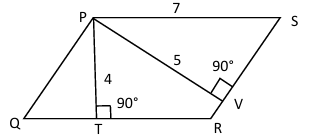
\includegraphics[width=0.3\linewidth]{figs/q3.png}
    \caption{}
    \label{fig:q3}
\end{figure}
\begin{multicols}{4}
\begin{enumerate}
\item $\frac{20}{7}$
\item $\frac{28}{5}$
\item $\frac{9}{2}$
\item $\frac{35}{4}$
\end{enumerate}
\end{multicols}

\item In 2022, June Huh was awarded the Fields medal, which is the highest prize in Mathematics. When he was younger, he was also a poet. He did not win any medals in the International Mathematics Olympiads. He dropped out of college. Based only on the above information, which one of the following statements can be logically inferred with certainty?
\begin{multicols}{2}
\begin{enumerate}
\item Every Fields medalist has won a medal in an International Mathematics Olympiad.
\item Everyone who has dropped out of college has won the Fields medal.
\item All Fields medalists are part-time poets.
\item Some Fields medalists have dropped out of college.
\end{enumerate}
\end{multicols}

\item A line of symmetry is defined as a line that divides a figure into two parts in a way such that each part is a mirror image of the other part about that line. The given figure consists of 16 unit squares arranged as shown. In addition to the three black squares, what is the minimum number of squares that must be coloured black, such that both PQ and MN form lines of symmetry? (The figure is representative)
\begin{figure}[H]
    \centering
    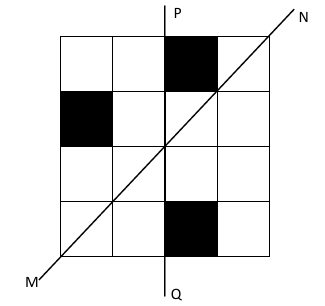
\includegraphics[width=0.3\linewidth]{figs/q5.png}
    \caption{}
    \label{fig:q5}
\end{figure}
\begin{multicols}{4}
\begin{enumerate}
\item 3
\item 4
\item 5
\item 6
\end{enumerate}
\end{multicols}

\subsection*{Q.6 - Q.10 carry two marks each.}

\item Human beings are one among many creatures that inhabit an imagined world. In this imagined world, some creatures are cruel. If in this imagined world, it is given that the statement ``Some human beings are not cruel creatures'' is FALSE, then which of the following set of statement(s) can be logically inferred with certainty? 
(i) All human beings are cruel creatures.
(ii) Some human beings are cruel creatures.
(iii) Some creatures that are cruel are human beings.
(iv) No human beings are cruel creatures.
\begin{multicols}{4}
\begin{enumerate}
\item only (i)
\item only (iii) and (iv)
\item only (i) and (ii)
\item (i), (ii) and (iii)
\end{enumerate}
\end{multicols}

\item To construct a wall, sand and cement are mixed in the ratio of 3:1. The cost of sand and that of cement are in the ratio of 1:2. If the total cost of sand and cement to construct the wall is 1000 rupees, then what is the cost (in rupees) of cement used?
\begin{multicols}{4}
\begin{enumerate}
\item 400
\item 600
\item 800
\item 200
\end{enumerate}
\end{multicols}

\item The World Bank has declared that it does not plan to offer new financing to Sri Lanka, which is battling its worst economic crisis in decades, until the country has an adequate macroeconomic policy framework in place. In a statement, the World Bank said Sri Lanka needed to adopt structural reforms that focus on economic stabilisation and tackle the root causes of its crisis. The latter has starved it of foreign exchange and led to shortages of food, fuel, and medicines. The bank is repurposing resources under existing loans to help alleviate shortages of essential items such as medicine, cooking gas, fertiliser, meals for children, and cash for vulnerable households. Based only on the above passage, which one of the following statements can be inferred with certainty?
\begin{multicols}{2}
\begin{enumerate}
\item According to the World Bank, the root cause of Sri Lanka’s economic crisis is that it does not have enough foreign exchange.
\item The World Bank has stated that it will advise the Sri Lankan government about how to tackle the root causes of its economic crisis.
\item According to the World Bank, Sri Lanka does not yet have an adequate macroeconomic policy framework.
\item The World Bank has stated that it will provide Sri Lanka with additional funds for essentials such as food, fuel, and medicines.
\end{enumerate}
\end{multicols}

\item The coefficient of $x^4$ in the polynomial $(x - 1)^3(x - 2)^3$ is equal to \underline{\hspace{1.5cm}}.
\begin{multicols}{4}
\begin{enumerate}
\item 33
\item $-3$
\item 30
\item 21
\end{enumerate}
\end{multicols}

\item Which one of the following shapes can be used to tile (completely cover by repeating) a flat plane, extending to infinity in all directions, without leaving any empty spaces in between them? The copies of the shape used to tile are identical and are not allowed to overlap.
\begin{multicols}{4}
\begin{enumerate}
\item circle
\item regular octagon
\item regular pentagon
\item rhombus
\end{enumerate}
\end{multicols}
\end{enumerate}

\section*{Aerospace Engineering (AE)}
\subsection*{Q.11 - Q.35 carry one mark each.}

\begin{enumerate}[leftmargin=*, resume]
\item The direction in which a scalar field $\phi(x, y, z)$ has the largest rate of change at any point with position vector $\vec{r} = x\hat{i} + y\hat{j} + z\hat{k}$ is the same as that of the vector
\begin{multicols}{2}
\begin{enumerate}
\item $\nabla\phi$
\item $\nabla \times (\psi\vec{r})$
\item $\psi\vec{r}$
\item $(\nabla\phi \cdot d\vec{r})\vec{r}$
\end{enumerate}
\end{multicols}

\item If a monotonic and continuous function $y = f(x)$ has only one root in the interval $x_1 < x < x_2$, then
\begin{multicols}{4}
\begin{enumerate}
\item $f(x_1)f(x_2) > 0$
\item $f(x_1)f(x_2) = 0$
\item $f(x_1)f(x_2) < 0$
\item $f(x_1) - f(x_2) = 0$
\end{enumerate}
\end{multicols}

\item Consider the one-dimensional wave equation $\frac{\partial u}{\partial t} + \frac{\partial u}{\partial x} = 0$ for $-\infty < x < \infty$, $t \geq 0$. For an initial condition $u(x,0) = e^{-x^2}$, the solution at $t = 1$ is
\begin{multicols}{2}
\begin{enumerate}
\item $u(x,1) = e^{-(x-1)^2}$
\item $u(x,1) = e^{-1}$
\item $u(x,1) = e^{-x^2}$
\item $u(x,1) = e^{-(x+1)^2}$
\end{enumerate}
\end{multicols}

\item A two-dimensional potential flow solution for flow past an airfoil has a streamline pattern as shown in the figure. Which of the following conditions is additionally required to satisfy the Kutta condition?
\begin{figure}[H]
    \centering
    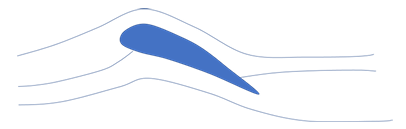
\includegraphics[width=0.5\linewidth]{figs/q14.png}
    \caption{}
    \label{fig:q14}
\end{figure}
\begin{multicols}{2}
\begin{enumerate}
\item Addition of a source of strength $Q > 0$
\item Addition of a source of strength $Q < 0$
\item Addition of a circulation of strength $\Gamma > 0$ (counter-clockwise)
\item Addition of a circulation of strength $\Gamma < 0$ (clockwise)
\end{enumerate}
\end{multicols}

\item Consider the Blasius solution for the incompressible laminar flat plate boundary layer. Among the following options, select the correct relation for the development of the momentum thickness $\theta$ with distance $x$ from the leading edge along the length of the plate.
\begin{multicols}{4}
\begin{enumerate}
\item $\theta \propto x^{2/3}$
\item $\theta \propto x^{1/2}$
\item $\theta \propto x^{1/7}$
\item $\theta \propto x^{-2/3}$
\end{enumerate}
\end{multicols}

\item In a two-dimensional potential flow, the doublet is a limit of the superposition of
\begin{multicols}{2}
\begin{enumerate}
\item a uniform stream and a source
\item a source and a sink of equal strength
\item a uniform stream and a sink
\item a source and a vortex
\end{enumerate}
\end{multicols}

\item An ideal glider has drag characteristics given by $C_D = C_{D0} + C_{Di}$, where $C_{Di} = KC_L^2$ is the induced drag coefficient, $C_L$ is the lift coefficient, and $K$ is a constant. For maximum range of the glider, the ratio $C_{D0}/C_{Di}$ is
\begin{multicols}{4}
\begin{enumerate}
\item 1
\item $\frac{1}{3}$
\item 3
\item $\frac{3}{2}$
\end{enumerate}
\end{multicols}

\item The figures shown in the options are schematics of airfoil shapes (not to scale). For a civilian transport aircraft designed for a cruise Mach number of 0.8, which among them is aerodynamically best suited as a wing section?
\begin{multicols}{4}
\begin{enumerate}
\item Option A
\item Option B
\item Option C
\item Option D
\end{enumerate}
\end{multicols}

\item For a longitudinally statically stable aircraft, which one of the following represents the relationship between the coefficient of pitching moment about the center of gravity $C_{m_{cg}}$ and absolute angle of attack $\alpha_a$? (Note: nose-up moment is positive.)
\begin{multicols}{2}
\begin{enumerate}
\item Graph A
\item Graph B
\item Graph C
\item Graph D
\end{enumerate}
\end{multicols}

\item In a single-spool aviation turbojet engine, which of the following is the correct relationship between the total work output $W_T$ of a 2-stage axial turbine and the total work required $W_C$ by a 6-stage axial compressor, neglecting losses?
\begin{multicols}{4}
\begin{enumerate}
\item $W_T = 2W_C$
\item $W_T = 6W_C$
\item $W_T = W_C$
\item $W_T = 3W_C$
\end{enumerate}
\end{multicols}

\item For a stage of a 50\% reaction ideal axial flow compressor (symmetrical blading), select the correct statement from the options given.
\begin{multicols}{2}
\begin{enumerate}
\item The stagnation enthalpy rise across the rotor is 50\% of the rise across the stage.
\item The static enthalpy rise across the rotor is 50\% of the rise across the stage.
\item Axial velocity component of the flow at the rotor exit is 50\% of that at the rotor entry.
\item The static pressure rise across the rotor is 50\% of the rise across the stator.
\end{enumerate}
\end{multicols}

\item An aircraft is cruising with a forward speed $V_a$ and the jet exhaust speed relative to the engine at the exit is $V_j$. If $V_j/V_a = 2$, what is the propulsive efficiency?
\begin{multicols}{4}
\begin{enumerate}
\item 0.50
\item 1.00
\item 0.33
\item 0.67
\end{enumerate}
\end{multicols}

\item Consider the four basic symmetrical flight loading conditions corresponding to the corners of a typical V-n diagram. For one of these flight loading conditions, it is observed that (i) the compressive bending stresses have a maximum value in the bottom aft region (see figure) of the wing cross-section; and (ii) the tensile bending stresses are maximum in the upper forward region (see figure) of the wing cross-section. For the preceding observations, select the corresponding flight loading condition from the options given.
\begin{figure}[H]
    \centering
    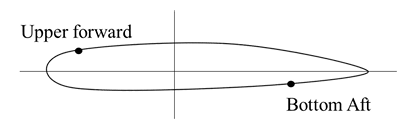
\includegraphics[width=0.5\linewidth]{figs/q23.png}
    \caption{}
    \label{fig:q23}
\end{figure}
\begin{multicols}{2}
\begin{enumerate}
\item Positive high angle of attack
\item Positive low angle of attack
\item Negative high angle of attack
\item Negative low angle of attack
\end{enumerate}
\end{multicols}

\item Which one of the following figures represents the qualitative variation of absolute deceleration with altitude $h$ (measured from the mean sea level) for a space vehicle undergoing a ballistic entry into the Earth’s atmosphere?
\begin{multicols}{4}
\begin{enumerate}
\item Figure A
\item Figure B
\item Figure C
\item Figure D
\end{enumerate}
\end{multicols}

\item Which of the following statement(s) is/are true about harmonically excited forced vibration of a single degree-of-freedom linear spring-mass-damper system?
\begin{enumerate}
\item The total response of the mass is a combination of free vibration transient and steady-state response.
\item The free vibration transient dies out with time for each of the three possible conditions of damping (under-damped, critically damped, and over-damped).
\item The steady-state periodic response is dependent on the initial conditions at the time of application of external forcing.
\item The rate of decay of free vibration transient response depends on the mass, spring stiffness and damping constant.
\end{enumerate}
\begin{multicols}{4}
\begin{enumerate}
\item A and B only
\item A, B and D only
\item B and C only
\item A, C and D only
\end{enumerate}
\end{multicols}

\item Which of the following statement(s) is/are true about the state of stress in a plane?
\begin{enumerate}
\item Maximum or major principal stress is algebraically the largest direct stress at a point.
\item The magnitude of minor principal stress cannot be greater than the magnitude of major principal stress.
\item The planes of maximum shear stress are inclined at 90 degrees to the principal axes.
\item The normal stresses along the planes of maximum shear stress are equal.
\end{enumerate}
\begin{multicols}{4}
\begin{enumerate}
\item A and B only
\item A, B and C only
\item B and D only
\item A, C and D only
\end{enumerate}
\end{multicols}

\item Which of the following statement(s) is/are true about the ribs of an airplane wing with semi-monocoque construction?
\begin{enumerate}
\item For a rectangular planform wing, the dimensions of the ribs DO NOT depend on their spanwise position in the wing.
\item Ribs increase the column buckling stress of longitudinal stiffeners connected to them.
\item Ribs increase plate buckling stress of the skin panels.
\item Ribs help in maintaining aerodynamic shape of the wing.
\end{enumerate}
\begin{multicols}{4}
\begin{enumerate}
\item B and D only
\item A, C and D only
\item B, C and D only
\item A, B and C only
\end{enumerate}
\end{multicols}

\item From the options given, select all that are true for turbofan engines with afterburners.
\begin{enumerate}
\item Turning afterburner ON increases specific fuel consumption.
\item Turbofan engines with afterburners have variable area nozzles.
\item Turning afterburner ON decreases specific fuel consumption.
\item Turning afterburner ON increases stagnation pressure across the engine.
\end{enumerate}
\begin{multicols}{4}
\begin{enumerate}
\item A and B only
\item B and C only
\item C and D only
\item A and D only
\end{enumerate}
\end{multicols}

\item Which of the following statement(s) is/are true with respect to eigenvalues and eigenvectors of a matrix?
\begin{enumerate}
\item The sum of the eigenvalues of a matrix equals the sum of the elements of the principal diagonal.
\item If $\lambda$ is an eigenvalue of a matrix A, then $\frac{1}{\lambda}$ is always an eigenvalue of its transpose ($A^T$).
\item If $\lambda$ is an eigenvalue of an orthogonal matrix A, then $\frac{1}{\lambda}$ is also an eigenvalue of A.
\item If a matrix has $n$ distinct eigenvalues, it also has $n$ independent eigenvectors.
\end{enumerate}
\begin{multicols}{4}
\begin{enumerate}
\item A and D only
\item B and C only
\item C and D only
\item A and B only
\end{enumerate}
\end{multicols}

\item For studying wing vibrations, a wing of mass M and finite dimensions has been idealized by assuming it to be supported using a linear spring of equivalent stiffness k and a torsional spring of equivalent stiffness $k_\theta$ as shown in the figure. The centre of gravity (CG) of the wing idealized as an airfoil is marked in the figure. The number of degree(s) of freedom for this idealized wing vibration model is \underline{\hspace{1.5cm}}. (Answer in integer)
\begin{figure}[H]
    \centering
    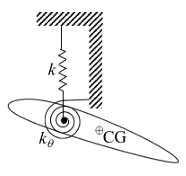
\includegraphics[width=0.3\linewidth]{figs/q30.png}
    \caption{}
    \label{fig:q30}
\end{figure}

\item The system of equations 
\begin{align*}
x - 2y + \alpha z &= 0 \\
2x + y - 4z &= 0 \\
x - y + z &= 0
\end{align*}
has a non-trivial solution for $\alpha =$ \underline{\hspace{1.5cm}}. (Answer in integer)

\item An airplane weighing 40 kN is landing on a horizontal runway during which it is retarded by an arresting cable mechanism. The tension in the arresting cable at a given instant, as shown in the figure, is 100 kN. Assuming that the thrust from the engine continues to balance airplane drag, the magnitude of horizontal load factor is \underline{\hspace{1.5cm}}. (round off to one decimal place)
\begin{figure}[H]
    \centering
    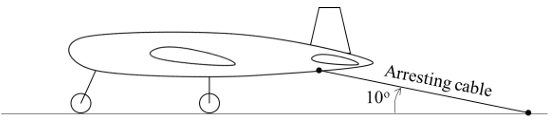
\includegraphics[width=0.3\linewidth]{figs/q32.png}
    \caption{}
    \label{fig:q32}
\end{figure}

\item The ratio of the speed of sound in H$_2$ (molecular weight 2 kg/kmol) to that in N$_2$ (molecular weight 28 kg/kmol) at temperature 300 K and pressure 2 bar is \underline{\hspace{1.5cm}}. (round off to two decimal places)

\item Airplane A and Airplane B are cruising at altitudes of 2 km and 4 km, respectively. The free stream density and static pressure at altitude 2 km are 1.01 kg/m$^3$ and 79.50 kPa, respectively, and at altitude 4 km, they are 0.82 kg/m$^3$ and 61.70 kPa, respectively. The differential pressure reading from the pitot-static tubes is 3 kPa for both the airplanes. Assuming incompressible flow, the ratio of cruise speeds of Airplane A to Airplane B is \underline{\hspace{1.5cm}}. (round off to two decimal places)

\item A supersonic vehicle powered by a ramjet engine is cruising at a speed of 1000 m/s. The ramjet engine burns hydrogen in a subsonic combustor to produce thrust. The heat of combustion for hydrogen is 120 MJ/kg. The overall efficiency of the engine $\eta_0$, defined as the ratio of propulsive power to the total heat release in the combustor, is 40\%. Taking acceleration due to gravity $g_0 = 10$ m/s$^2$, the specific impulse of the engine is \underline{\hspace{1.5cm}} seconds. (round off to the nearest integer)

\subsection*{Q.36 - Q.65 carry two marks each.}

\item Given the function $y(x) = (x + 3)(x - 2)$, for $-4 < x < 4$. What is the value of $x$ at which the function has a minimum?
\begin{multicols}{4}
\begin{enumerate}
\item $-\frac{3}{2}$
\item $-\frac{1}{2}$
\item $\frac{1}{2}$
\item $\frac{3}{2}$
\end{enumerate}
\end{multicols}

\item A supersonic aircraft has an air intake ramp that can be rotated about the leading edge O such that the shock from the leading edge meets the cowl lip as shown in the figure. Select all the correct statement(s) as per oblique shock theory when the flight Mach number M is increased.
\begin{figure}[H]
    \centering
    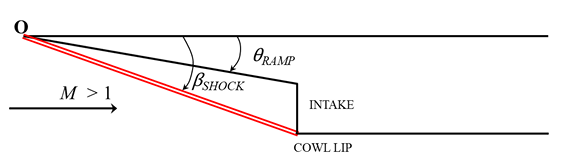
\includegraphics[width=0.3\linewidth]{figs/q37.png}
    \caption{}
    \label{fig:q37}
\end{figure}
\begin{enumerate}
\item It is always possible to find a ramp setting $\theta_{RAMP}$ such that the shock still meets the cowl lip ($\beta_{SHOCK}$ remains the same).
\item If $\theta_{RAMP}$ is held fixed, the shock angle $\beta_{SHOCK}$ will increase.
\item If M exceeds a critical value, it would NOT be possible to find a ramp setting $\theta_{RAMP}$ such that the shock still meets the cowl lip ($\beta_{SHOCK}$ remains the same).
\item Shock angle $\beta_{SHOCK} < \sin^{-1}\left(\frac{1}{M}\right)$
\end{enumerate}
\begin{multicols}{4}
\begin{enumerate}
\item A and B only
\item B and C only
\item C and D only
\item A and D only
\end{enumerate}
\end{multicols}

\item Two missiles A and B powered by solid rocket motors have identical specific impulse, liftoff mass of 5600 kg each, and burn durations of $t_A = 30$ s and $t_B = 70$ s, respectively. The propellant mass flow rates, $\dot{m}_A$ and $\dot{m}_B$, for missiles A and B, respectively, are given by
\[
\dot{m}_A = 120 \text{ kg/s}, \quad 0 \leq t \leq 30
\]
\[
\dot{m}_B = 70 \text{ kg/s}, \quad 0 \leq t \leq 70
\]
Neglecting gravity and aerodynamic forces, the relationship between the final velocities $V_A$ and $V_B$ of missiles A and B, respectively, is given by
\begin{multicols}{4}
\begin{enumerate}
\item $V_A = 4.1 V_B$
\item $V_A = V_B$
\item $V_A = 0.5 V_B$
\item $V_A = 0.7 V_B$
\end{enumerate}
\end{multicols}

\item A perfect gas stored in a large reservoir exhausts into the atmosphere through a convergent duct. The reservoir pressure is $P_0$ and temperature is $T_0$. The jet emerges from the nozzle at choked conditions with average velocity $u$, Mach number $M$, pressure $p$, temperature $T$, and density $\rho$. If the reservoir pressure is increased, then
\begin{multicols}{2}
\begin{enumerate}
\item $u$, $M$, $p$, $T$, and $\rho$ increase
\item $u$, $p$, $T$, and $\rho$ increase, but $M$ remains the same
\item $u$, $M$, and $T$ remain the same, but $p$ and $\rho$ increase
\item $u$, $M$, $T$ and $\rho$ remain the same, but $p$ increases
\end{enumerate}
\end{multicols}

\item Consider a general aviation airplane with weight 10 kN and a wing planform area of 15 m$^2$. The drag coefficient of the airplane is given as $C_D = C_{D0} + K C_L^2$ with $C_{D0} = 0.025$ and $K = 0.05$. For level flight at an altitude where the density is 0.60 kg/m$^3$ and thrust 1 kN, the maximum cruise speed is (rounded off to the nearest integer)
\begin{multicols}{4}
\begin{enumerate}
\item 87 m/s
\item 30 m/s
\item 36 m/s
\item 101 m/s
\end{enumerate}
\end{multicols}

\item A scramjet engine features an intake, isolator, combustor, and a nozzle, as shown in the schematic. Station 3 indicates the combustor entry point. Assume stagnation enthalpy to be constant between Stations 1 and 3, and air to be a calorically perfect gas with specific heat ratio $\gamma$. Select the correct expression for Mach number $M_3$ at the inlet to the combustor from the options given.
\begin{figure}[H]
    \centering
    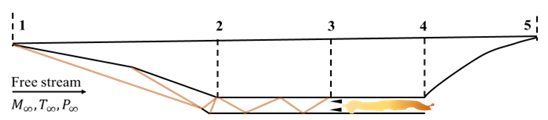
\includegraphics[width=0.3\linewidth]{figs/q41.png}
    \caption{}
    \label{fig:q41}
\end{figure}
\begin{multicols}{2}
\begin{enumerate}
\item $M_3 = M_\infty \sqrt{\frac{T_\infty}{T_3} - 1}(\gamma - 1)$
\item $M_3 = \sqrt{\frac{(\gamma - 1)\left[1 + \frac{\gamma - 1}{2}M_\infty^2\right]\frac{T_\infty}{T_3} - 1}{\frac{\gamma - 1}{2}}}$
\item $M_3 = M_\infty \sqrt{\frac{T_\infty}{T_3}}$
\item $M_3 = \sqrt{\frac{\frac{\gamma + 1}{2}\frac{T_\infty}{T_3} - 1}{\frac{\gamma - 1}{2}}}$
\end{enumerate}
\end{multicols}

\item Consider the equation $\frac{dy}{dx} + a y = \sin(\omega x)$, where $a$ and $\omega$ are constants. Given $y = 1$ at $x = 0$, select all correct statement(s) from the following as $x \to \infty$.
\begin{enumerate}
\item $y \to 0$ if $a \neq 0$
\item $y \to 1$ if $a = 0$
\item $y \to A \exp(|a|x)$ if $a < 0$; $A$ is a constant
\item $y \to B \sin(\omega x + C)$ if $a > 0$; $B$ and $C$ are constants
\end{enumerate}
\begin{multicols}{4}
\begin{enumerate}
\item A and B only
\item B and C only
\item C and D only
\item A and D only
\end{enumerate}
\end{multicols}

\item Given the vectors 
\begin{align*}
\vec{A} &= 9\hat{i} - 5\hat{j} + 2\hat{k} \\
\vec{B} &= 11\hat{i} + 4\hat{j} + \hat{k} \\
\vec{C} &= -7\hat{i} + 14\hat{j} - 3\hat{k}
\end{align*}
which of the following statement(s) is/are TRUE?
\begin{enumerate}
\item Vectors $\vec{A}$, $\vec{B}$ and $\vec{C}$ are coplanar
\item The scalar triple product of the vectors $\vec{A}$, $\vec{B}$ and $\vec{C}$ is zero
\item $\vec{A}$ and $\vec{B}$ are perpendicular
\item $\vec{C}$ is parallel to $\vec{A} \times \vec{B}$
\end{enumerate}
\begin{multicols}{4}
\begin{enumerate}
\item A and B only
\item B and C only
\item C and D only
\item A and D only
\end{enumerate}
\end{multicols}

\item Consider a one-dimensional inviscid supersonic flow in a diverging duct with heat addition ($Q_{in}$) as shown. Which of the following statement(s) is/are always TRUE?
\begin{figure}[H]
    \centering
    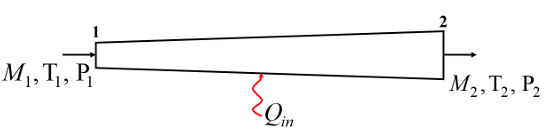
\includegraphics[width=0.3\linewidth]{figs/Q44.png}
    \caption{}
    \label{fig:q44}
\end{figure}
\begin{enumerate}
\item Mach number, $M_2 > M_1$
\item Stagnation pressure, $P_1^0 > P_2^0$
\item Static pressure, $P_2 > P_1$
\item Stagnation temperature, $T_1^0 < T_2^0$
\end{enumerate}
\begin{multicols}{4}
\begin{enumerate}
\item A and B only
\item B and C only
\item C and D only
\item A and D only
\end{enumerate}
\end{multicols}

\item Consider the International Standard Atmosphere (ISA) with $h$ being the geopotential altitude (in km) and $\frac{dT}{dh}$ being the temperature gradient (in K/m). Which of the following combination(s) of $\left(h, \frac{dT}{dh}\right)$ is/are as per ISA?
\begin{enumerate}
\item $(7, -6.5 \times 10^{-3})$
\item $(9, 4 \times 10^{-3})$
\item $(15, 0)$
\item $(35, 3 \times 10^{-3})$
\end{enumerate}
\begin{multicols}{4}
\begin{enumerate}
\item A and C only
\item B and D only
\item C and D only
\item A and B only
\end{enumerate}
\end{multicols}

\item For an airfoil, which of the relations given about the critical Mach number $M_{cr}$ and drag divergence Mach number $M_{dd}$ is/are correct?
\begin{enumerate}
\item $M_{cr} < M_{dd}$
\item $M_{cr} < 1.0$
\item $M_{dd} < 1.0$
\item $M_{cr} > 1.0$
\end{enumerate}
\begin{multicols}{4}
\begin{enumerate}
\item A and B only
\item B and C only
\item C and D only
\item A and D only
\end{enumerate}
\end{multicols}

\item Which of the following statement(s) about the elastic flexural buckling load of columns is/are correct?
\begin{enumerate}
\item The buckling load increases with increase in flexural rigidity of the column.
\item The buckling load increases with increase in the length of the column.
\item The boundary conditions of the column affect the buckling load.
\item The buckling load is NOT directly dependent on the density of the material used for the column.
\end{enumerate}
\begin{multicols}{4}
\begin{enumerate}
\item A and C only
\item B and D only
\item C and D only
\item A and B only
\end{enumerate}
\end{multicols}

\item The thickness of a uniform hollow circular shaft is equal to the difference between the outer radius and the inner radius. The ratio of the inner diameter to outer diameter of the shaft is 0.5. For the shaft reacting to an applied torque, the ratio of the maximum shear stress $\tau$ to the maximum shear stress $\tau_{\text{thin-wall}}$ obtained using the thin-wall approximation is \underline{\hspace{1.5cm}}. (round off to one decimal place)

\item A rigid bar AB is subjected to a uniformly distributed load of 100 N/m as shown in the figure. The bar is supported by rod CD, with A, C, and D as pin joints. The rod CD has axial stiffness of 40 N/mm. The vertical deflection at point D is \underline{\hspace{1.5cm}} mm. (round off to nearest integer)
\begin{figure}[H]
    \centering
    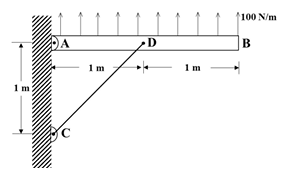
\includegraphics[width=0.3\linewidth]{figs/q49.png}
    \caption{}
    \label{fig:q49}
\end{figure}

\item A cantilever beam of length 2a is loaded at the tip with force F as shown in the figure. The beam is supported in the middle by a roller with a pin. The magnitude of moment reaction at the built-in end of the beam is $\mathbb{C} Fa$, where $\mathbb{C}$ is \underline{\hspace{1.5cm}}. (round off to one decimal place)
\begin{figure}[H]
    \centering
    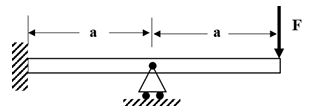
\includegraphics[width=0.5\linewidth]{figs/q50.png}
    \caption{}
    \label{fig:q50}
\end{figure}

\item A single degree-of-freedom spring-mass-damper system has viscous damping ratio of 0.1. The mass is given an initial displacement of 10 cm without imparting any velocity. After exactly two complete cycles of oscillation (i.e., after time $2T_d$, where $T_d$ is the period of the damped vibration), the amplitude of the displacement is \underline{\hspace{1.5cm}} cm. (round off to two decimal place)

\item The shear flow distribution in a single cell, thin-walled beam under the action of an arbitrary shear load $S_y$ applied at the shear centre S is shown in the figure. The cell has horizontal symmetry with booms marked by 1 to 4 that carry direct stresses. The shear modulus G is the same for all the walls, and the area of the cell is 135000 mm$^2$. With respect to the point O marked in the figure, the distance to the shear centre S is \underline{\hspace{1.5cm}} mm. (round off to the nearest integer)
\begin{figure}[H]
    \centering
    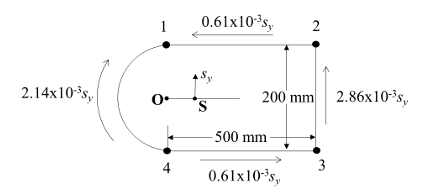
\includegraphics[width=0.5\linewidth]{figs/q52.png}
    \caption{}
    \label{fig:q52}
\end{figure}

\item Consider a thin-walled cylindrical pressure vessel made of an alloy with yield strength of 300 MPa. The vessel has end caps to contain the pressure. The ratio of radius of the vessel to its wall thickness is 100. As per the von Mises yield criterion, the internal pressure that would cause the failure of the vessel is \underline{\hspace{1.5cm}} MPa. (round off to two decimal places)

\item Consider the differential equation $x^2 \frac{d^2y}{dx^2} + 4x \frac{dy}{dx} + 2y = 0$ for $x \geq 1$ with initial conditions $y = 0$, $\frac{dy}{dx} = 1$ at $x = 1$. The value of $y$ at $x = 2$ is \underline{\hspace{1.5cm}}. (round off to two decimal places)

\item The operating characteristics of a pump were measured to be $C_P = a \Phi^2$, where power coefficient $C_P = \frac{P}{\rho \omega^3 D^5}$, $\Phi$ is the flow coefficient, $a$ is a constant, $D$ is a length scale, $\omega$ is the rotation rate, $\rho$ is fluid density, and $P$ is the power required. The flow coefficient is a dimensionless volume flow rate scaled with $\omega$ and $D$. Assuming that the flow rate remains the same, if the rotation rate is increased to 1.25 $\omega$, the power changes to $\alpha P$. The value of $\alpha$ is \underline{\hspace{1.5cm}}. (round off to two decimal places)

\item A thin cambered airfoil has lift coefficient $c_l = 0$ at an angle of attack $\alpha = -1.1^\circ$. Assuming that stall occurs at much larger $\alpha$, the $c_l$ at $\alpha = 4^\circ$ is \underline{\hspace{1.5cm}}. (round off to two decimal places)

\item In a potential flow, a uniform stream of strength $U$ directed along the x-axis and four line sources (2-dimensional) of strengths $\frac{\pi}{2}, -\frac{\pi}{3}, \frac{\pi}{4}, -\frac{\pi}{5}$ are placed along the x-axis at $x = 0, 1, 2$ and 3, respectively. The strength of an additional line source to be placed at $x = 4$ such that a closed streamline encircles all five sources is \underline{\hspace{1.5cm}}. (round off to two decimal places)

\item Enstrophy is defined as the square of the magnitude of vorticity. For the three-dimensional velocity field
\[
\vec{V} = (4x - 1.5y + 2.5z)\hat{i} + (1.5x - 1.5y)\hat{j} + (0.7xy)\hat{k},
\]
the enstrophy at location $(1, 1, 1)$ is \underline{\hspace{1.5cm}}. (round off to two decimal places)

\item An airplane with wing planform area of 20 m$^2$ and weight 8 kN is flying straight and level with a speed of 100 m/s. The total drag coefficient is 0.026 and the air density is 0.7 kg/m$^3$. The total thrust required to introduce a steady climb angle of 0.1 radians is \underline{\hspace{1.5cm}} N. (round off to the nearest integer)

\item The maximum permissible load factor and the maximum lift force coefficient for an airplane is 7 and 2, respectively. For a wing loading of 6500 N/m$^2$ and air density 1.23 kg/m$^3$, the speed yielding the highest possible turn rate in the vertical plane is \underline{\hspace{1.5cm}} m/s. (round off to the nearest integer)

\item A gas turbine combustor is burning methane and air at an equivalence ratio $\phi = 0.5$, where $\phi = \frac{F/A}{(F/A)_{\text{stolch}}}$ and $(F/A)_{\text{stolch}}$ is the ratio of mass flow rate of fuel to the mass flow rate of air at stoichiometry. If the air flow rate is $\dot{m}_{\text{air}} = 20$ kg/s then the mass flow rate of methane is \underline{\hspace{1.5cm}} kg/s. (round off to two decimal places)

\item The universal gravitational constant is $6.67 \times 10^{-11}$ Nm$^2$/kg$^2$. For a planet of mass $6.4169 \times 10^{23}$ kg and radius 3390 km, the escape velocity is \underline{\hspace{1.5cm}} km/s. (round off to one decimal place).

\item A satellite is in a circular orbit around Earth with a time period of 90 minutes. The radius of Earth is 6370 km, mass of Earth is $5.98 \times 10^{24}$ kg and the universal gravitational constant is $6.67 \times 10^{-11}$ Nm$^2$/kg$^2$. The altitude of the satellite above mean sea level is \underline{\hspace{1.5cm}} km. (round off to the nearest integer)

\item A centrifugal air compressor has inlet root diameter of 0.25 m and the outlet diameter of the impeller is 0.6 m. The pressure ratio is 5.0. The air at the inlet of the rotor is at 1 atm and 25°C. The polytropic efficiency is 0.8 and slip factor is 0.92. Use $C_p = 1.004$ kJ/kg-K and $\gamma = 1.4$. The impeller speed in revolutions per minute (RPM) is \underline{\hspace{1.5cm}}. (round off to the nearest integer)

\item Consider a cryogenic liquid rocket engine using an expander cycle with liquid hydrogen and liquid oxygen as the two propellants. The mass flow rate of hydrogen $\dot{m}_{H_2}$ into the combustion chamber is 32 kg/s, and the mass flow rate of oxygen $\dot{m}_{O_2}$ into the chamber is such that $\dot{m}_{O_2}/\dot{m}_{H_2} = 8$. The combustion of hydrogen and oxygen is at stoichiometry. Assuming that the rate of the forward reaction is much larger than that of the reverse reaction, the rate of formation of H$_2$O is \underline{\hspace{1.5cm}} kmol/s. (round off to the nearest integer)\\
\\
\large
\centering
\textbf{END OF THE QUESTION PAPER}

\end{enumerate}

\end{document}